According to the National Eye Institute (NEI), approximately 40,000 cornea transplants are performed every year in the United States. Unfortunately, about 20 percent (8000 per year) of these transplants are rejected~\citep{NEIcornea}, necessitating a second transplant. An increase in the number of procedures is inconvenient for the patient at best; therefore, it is desirable to find ways to minimize the amount of rejection as well as increase the overall supply of tissue for cornea transplants.

\section{Corneal Engineering}
\label{cornealengineering}

Prof. Liz Orwin's lab at Harvey Mudd College is attempting to overcome the challenges of cornea transplants by growing replacement corneas. This is done by electrospinning collagen fibers, then seeding cells from a patient who needs new corneas. However, the electrospun collagen does not possess the structural properties of corneal collagen, so the Orwin Lab is focused on finding ways to control the phenotype and regulatory mechanisms of the cells. It is hoped that through this process, the cells will reenact the initial formation of the corneas in fetal development, taking up the electrospun collagen and laying it back down in the native form, viz., a hexagonal close-packed array of 30 nm-diameter collagen fibrils.

In order to better understand the behavior of the cells in response to the treatments they receive, Prof. Orwin's lab would like to be able to monitor both the position and phenotype of the cells in the scaffold. Confocal microscopy, a standard biological imaging modality, has a high ($<1\,\mu$m isotropic) resolution but can only image 25 $\mu$m deep. The high resolution makes confocal desirable, but human corneas are 500 $\mu$m thick, and the collagen scaffolds can be thicker, making confocal unusable for full 3D imaging. In contrast, the optical coherence microscope (OCM) trades high resolution for moderate resolution ($5\,\mu$m lateral, $10\,\mu$m axial) and over 1 mm of depth penetration at 850 nm wavelength. Consequently, the OCM was employed to monitor the cells.

Unfortunately, the collagen in the scaffold scatters too highly for the OCM to distinguish the cells, so Chris Raub '04 proposed a method, developed from a paper by Sokolov~\citep{Sokolov}, wherein 35 nm gold nanoparticles would be applied to increase scattering of the cells via a process called indirect immunolabeling (see \autoref{indirectimmunolabeling})), the basic precepts of which are still used in this project~\citep{raub}. Indirect immunolabeling has four key components: a target protein (we are targeting $\alpha 5 \beta 1$-integrin), a primary antibody (MAB1999) that is \emph{anti}- the target protein, a secondary antibody (AP124F) that is \emph{anti}- the primary antibody, and a label (both the gold nanoparticles and a fluorescent molecule on the AP124F). Indirect immunolabeling is implemented by first binding primary antibodies specifically to their target proteins on the surfaces of corneal cells. Then, secondary antibodies (anti-Ab1) are bound to nanoparticles via van der Waals forces. The antibody-gold is then allowed to bind to the Ab1-protein-cell \emph{in vitro}. A schematic diagram of this process is shown in \autoref{indirectimmunolabeling}.

\begin{figure}[htbp]
\centering
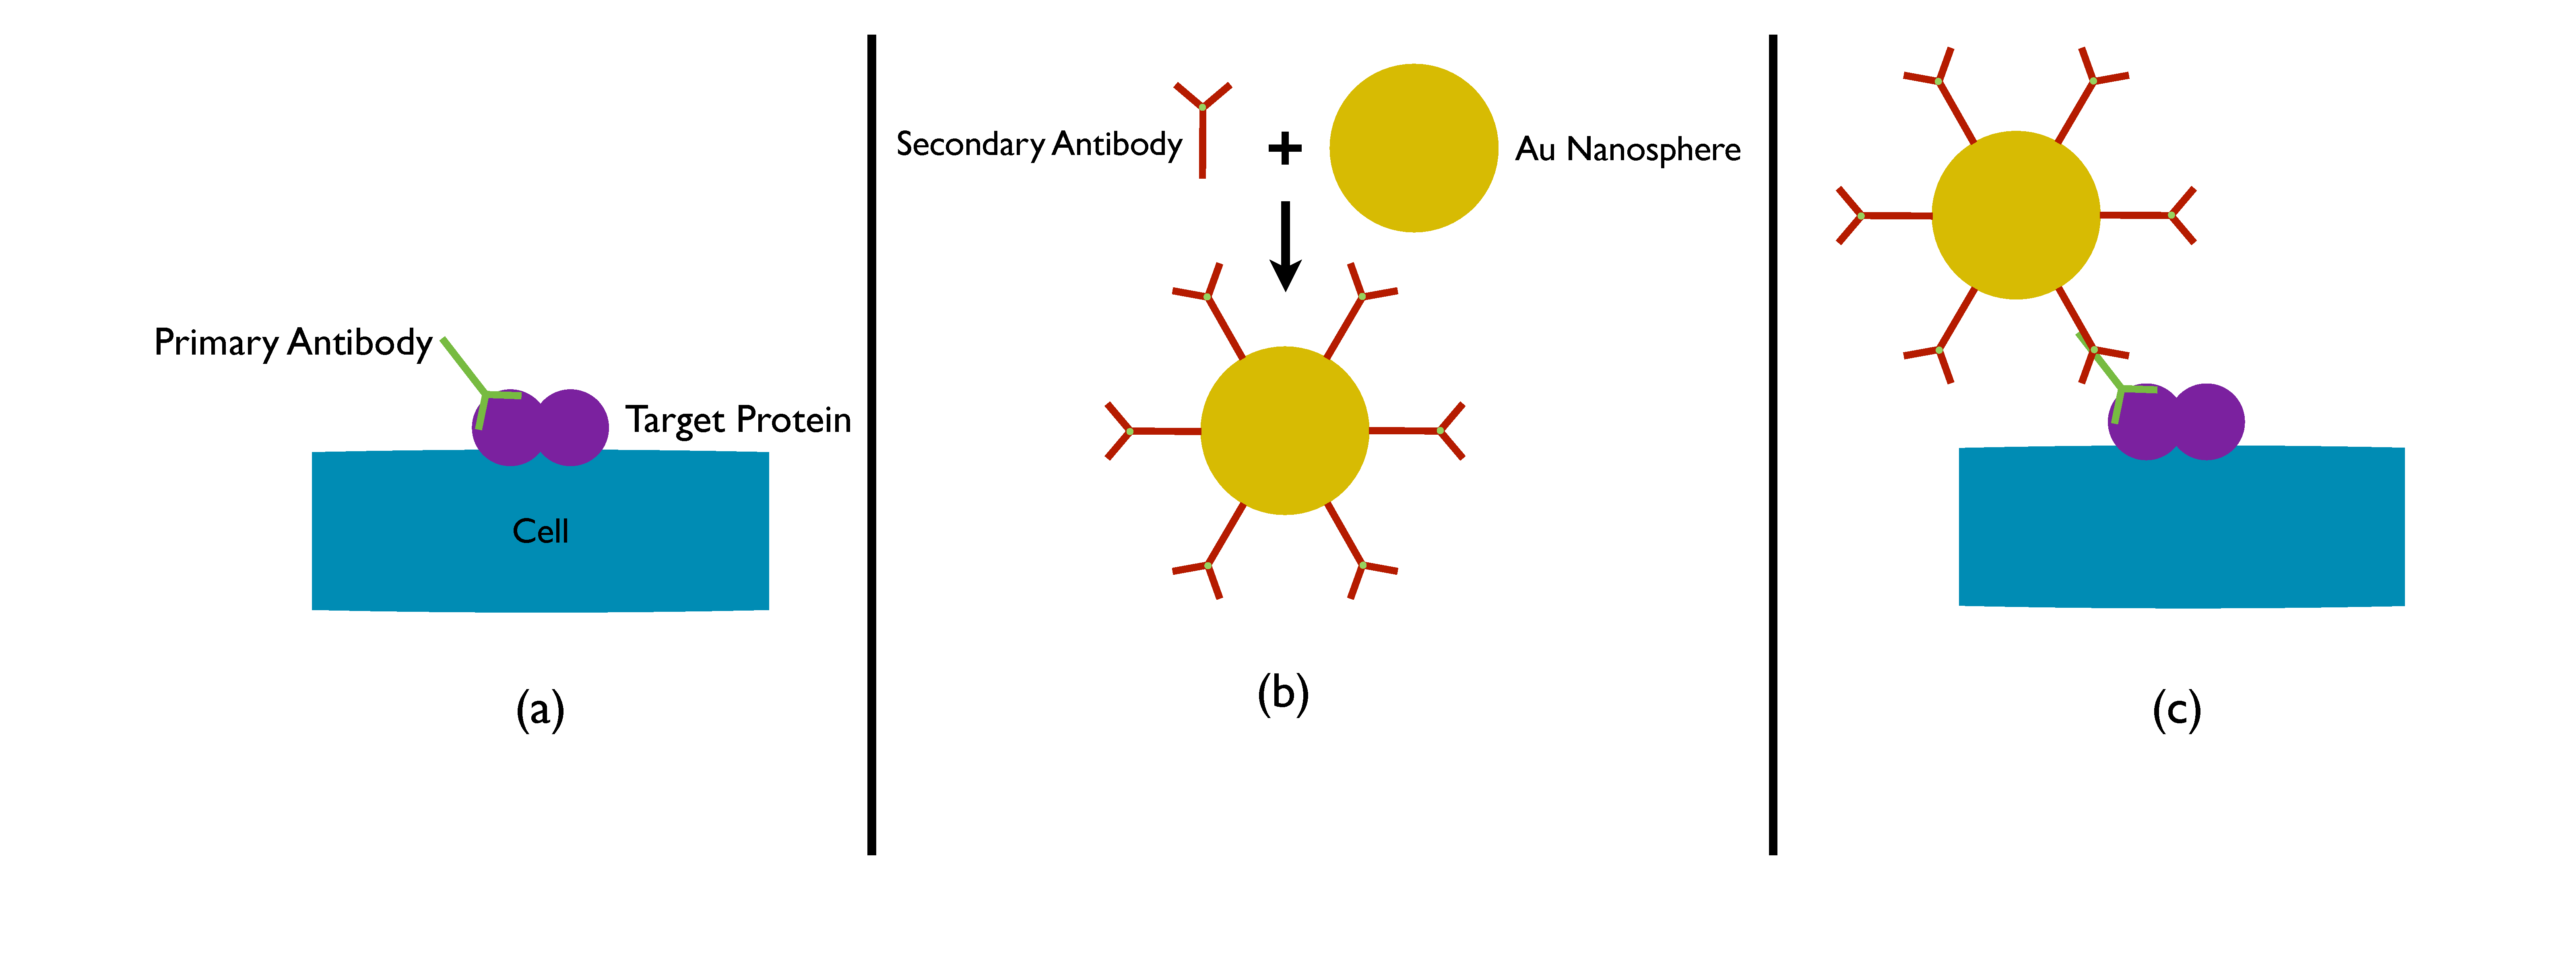
\includegraphics[keepaspectratio,width=\textwidth,height=0.75\textheight]{./IndirectImmunolabeling.pdf}
\caption{Stages of indirect immunolabeling presented schematically (not to scale). (a) The primary antibody, MAB1999, binds to the targeted surface protein, $\alpha 5 \beta 1$-integrin. (b) Secondary antibodies, AP124F, are bound to the surface of a gold nanoparticle. (c) A gold nanoparticle-secondary antibody complex binds to the primary antibody, which is in turn bound to the surface protein.}
\label{indirectimmunolabeling}
\end{figure}



Jamie Shoffeit '05~\citep{chanshoffeit}, Megan Arman '06, and Emily Hogan '07 all followed on Raub's work to achieve labeling. The process they employed consisted of creating 35 nm diameter gold nanoparticles from a citrate reduction of Au(III) and binding the antibodies to the nanoparticles via van der Waals forces alone. Although Hogan was finally able to use this technique to produce a statistically significant increase in scattering in 2007, the scattering increase was not as great as was desired.

To address this, David Coats '08 did a number of studies to optimize the gold being used as the labeling agent. Coats performed extensive calculations using Mie theory to maximize scattering. Mie theory details the scattering pattern of particles on the order of or larger than the wavelength of light they scatter. As even a 35 nm nanoparticle cannot be approximated as a point when using 850 nm light, Mie theory provides a far more accurate prediction of the intensity of backscattered intensity than Rayleigh scattering theory. These calculations showed that for any diameter, a particle made of solid gold (versus a particle with an inner core of silica) gave the highest scattering to absorption cross-section ratio, as shown in \autoref{whatcore}. As can also be seen in that image, $C_{sca}/C_{abs}$ also increases with diameter, up to a point. However, the settling rate of the gold particles also had to be taken into account, as well as the availability of manufactured gold nanoparticles. With these multiple factors in consideration, it was decided that 90 nm diameter nanoparticles from Nanopartz would be used. With these improved gold particles, David Coats again performed imaging tests on a monolayer of cells. However, the same lack of obvious signal generation prompted even further investigation.

\begin{figure}[htbp]
\centering
\includegraphics[keepaspectratio,width=4in,height=0.75\textheight]{CscaCabs.pdf}
\caption{Plot of the ratio of the scattering cross section $C_{sca}$ to the absorption cross section $C_{abs}$ as a function of total particle diameter, calculated via Mie theory. Line color, as indicated by legend, corresponds to percent of total diameter taken up by silica inner core. Index of refraction values used are $n_{\mathrm{Au}}=0.194 - 5.527i$, $n_{\mathrm{silica}}=1.44$, and $n_{\mathrm{water}}=1.33$ for the surrounding region. From reference~\citep{coats}.}
\label{whatcore}
\end{figure}



One concern regarding the labeling system was that the antibodies were bound to the gold with only van der Waals forces. Rob Warren '10~\citep{warren} discovered a procedure in a paper by Lowery et al.~\citep{westpegylation} by which increased binding had been achieved for immunolabeling. The procedure is called PEGylation because of its use of polyethylene glycol polymer chains; a schematic diagram of the process is shown in \autoref{pegylation}. The procedure consists of using a polyethylene glycol (PEG) polymer chain functionalized at one end with orthopyridyl disulfide (OPSS) and at the other with an N-Hydroxysuccinimide ester (NHS). The OPSS-PEG-NHS is incubated with the antibody for 24 hours, in which time the NHS ester reacts with a lysine in the antibody, leaving the NHS ester free in solution and the antibody attached to the OPSS-PEG. This OPAb, as we call it, is then incubated with the gold for 24 hours, so that the OPSS group splits at the disulfide bond and the PEG chain attaches to the gold via a thiol bond, which has a strength slightly less than that of a covalent bond and much larger than that of a van der Waals bond !(appendix or footnote or reference on thiol bonds?). This should ensure that the antibody is firmly attached to the gold. The second part of the procedure is to prevent any other molecules from binding with the gold. This is accomplished by binding another PEG chain to the gold, of which one end is functionalized with a thiol group (SH) that then forms a thiol bond with the gold. This should fill any space left after the addition of the OPAb. 

\begin{figure}[htbp]
\centering
\includegraphics[keepaspectratio,width=\textwidth,height=0.75\textheight]{pegylation.jpg}
\caption{Schematic diagram of the PEGylation process. (a) The OPSS-PEG-NHS (OPN) binds to the antibody (Ab) to form OPAb. (b) The OPAb binds to the Au nanosphere to form OPAb-Au. (c) The PEG-SH fills in the gaps on the surface of the OPAb-Au, forming OPAb-Au-PS and protecting the sphere.}
\label{pegylation}
\end{figure}



Unfortunately, these tests also failed to produce the desired specific increase in scattering, so in the summer of 2010 Oliver Hoidn and Perry Ellis '11 undertook a reexamination of the PEGylation protocol. Several significant results emerged from their studies that indicated problems with the PEGylation protocol. First, the Nanopartz gold nanoparticle solution, though its pH is advertised as between 6 and 8, was actually measured at a pH between 5 and 5.5~\citep{hoidnellis} due to the lack of a buffer in the solution. However, if commercial PBS is added, the salt in that solution screens the negative capping agent on the gold nanoparticles, thus eliminating the mutual repulsion between the nanoparticles and causing them to agglomerate and fall out of solution. To remedy this, a buffer solution made of Na$_2$HPO$_4\cdot$7H$_2$O and NaH$_2$PO$_4\cdot$H$_2$O was added to the gold to achieve a total salt concentration of 10 mM. This concentration was chosen as it provides a sufficient level of buffering without screening the capping agent too much. However, over the course of the several days required for the full PEGylation process, it was found that the final immunolabeled gold nanoparticles still suffered from a high rate of agglomeration. A footnote was then found in Lowery et al.~\citep{westpegylation} that noted that PEG-SH cannot perform its protective function unless it has a molecular weight of at least 5 kDa. As the PEG-SH used up to that point had been of molecular weight 1.2 kDa, it had not protected the gold.

Thus, after Oliver and Perry concluded their work in the summer of 2010, it remained to readjust the PEGylation protocol for 5 kDa PEG-SH, and to use that updated protocol to once again try to significantly increased specific immunolabeling. In addition, it was discovered that the NHS ester used to bind the OPN to the antibody can undergo hydrolysis, rendering it incapable of binding; therefore, it was also necessary to examine the hydrolysis of the NHS ester. To date, the issue of NHS hydrolysis has been settled (\autoref{additionofantibodiestonanospheres}) and the PEGylation protocol has been optimized with the 5 kDa PEG-SH (\autoref{additionofpeg-shtonanospheres}). The optimized protocol produces strucural results consistent with the model of PEGylation we have developed (\autoref{resultsofthefullprotocol}). In addition, the 5 kDa PEG-SH appears to provide excellent long-term protection against agglomeration of the spheres. Spheres made with the optimized protocol have been used in two labeling experiments (\autoref{resultsofthe6marchlabelingsession} and \autoref{resultsofthe3aprillabelingsession}), which have provided further insights into the immunolabeling process.
